
%%%%%%%%%%%%%%%%%%%%%%%%%%%%%%%%%%%%%%%%%%%%%%%%%%%%%%%%%%%%%%%%%
% This is the main text file, in which all the sections of this report are called and compiled

%=================== Beginning ==================

\documentclass[12pt]{article}
\usepackage{graphicx}
\usepackage{fontspec}
\usepackage[utf8]{inputenc}
\usepackage[english]{babel}
% Calibri Font
\setromanfont[
BoldFont=CalibriBold.ttf,
ItalicFont=CalibriItalic.ttf,
BoldItalicFont=CalibriBoldItalic.ttf,
]{Calibri.ttf}

%=============== Margin
\usepackage{geometry}
\geometry{a4paper, left=22mm,  top=22mm, bottom=22mm, right=22mm}
%===============
\usepackage{setspace}
\usepackage[document]{ragged2e} % left-alignment
\hyphenpenalty=10000
\tolerance=10000
%--------------------------------
\usepackage{amsmath} % Mathematical Equations 

\begin{document}
\onehalfspacing

%===================== Cover =======================

\thispagestyle{empty} 
\begin{titlepage}
    \centering
    
\includegraphics[width=0.25\textwidth]{Figures/Logos/uom_logo.pdf}
    \hspace{170}
    
\includegraphics[width=0.35\textwidth]{Figures/Logos/Sheffield.pdf}
    \begin{center}
       \vspace*{4cm}
       {\LARGE Research Software Engineering Practice}
       \vspace{3cm}
    \begin{large}   
    

         
         \vspace{0.5cm}

        {\LARGE Analysis of the connectivity of hydrides within the microstructure of Zr alloys} \\

       \vspace{1.5cm}
        
        {\bf \today} \\
                
        
       \vspace{3 cm}
        Group 2 \\
       \textbf{Laura Gonzalez,
       Wunmi Olukoya,
       Jamie McGregor, 
       Enn Veikesaar }\\

       \vfill
       \centering
       
        {\bf \large Advanced Metallic System CDT Program}\\
          
        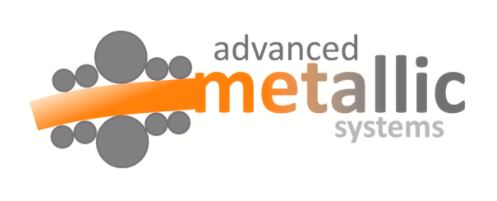
\includegraphics[width=0.35\textwidth]{Figures/CDT.JPG}
    
    \end{large}  
   \end{center}
\end{titlepage}

%===================== Abstract ==================

\section*{Abstract}

\justifying
\noindent
The presence of hydrides is a major concern in Zr alloys due to their embrittling effect. It has been observed that extent of embrittlement depends on the hydrides disposition and connectivity in the alloy. Therefore, characterizing their connectivity would allow the creation of tougher Zr alloys for nuclear applications. In this project, a model has been developed to evaluate the hydrides connectivity on Zr alloy microstructures. The model, developed with Python language, consists of loading up existing micrographs of Zr alloy microstructures, binarising them using different thresholding methods (otsu, k-means and adaptive Gauss thresholding) and obtaining the Hydride Continuity Coefficient (HCC) to study the hydrides connectivity. 

%=================== Table of Content ======================

\newpage
\begin{singlespacing}
\tableofcontents
\end{singlespacing}
\setlength{\parskip}{1em}
\renewcommand{\baselinestretch}{2.0}


%================= Start of the report ===================

\newpage 
\pagenumbering{arabic}
\setcounter{page}{1}
\onehalfspacing



%=================== Contributions =======================

\newpage 
\section*{Contributions}

Description of each team members role and contribution

\begin{enumerate}
\item Laura Gonzalez:
    \begin{enumerate}
          \item second level item
          \item second level item
    \end{enumerate}
\item Wunmi Olukoya:
        \begin{enumerate}
          \item second level item
          \item second level item
    \end{enumerate}
\item Jamie McGregor: 
        \begin{enumerate}
          \item second level item
          \item second level item
    \end{enumerate}
\item Enn Veikesaar:
        \begin{enumerate}
          \item second level item
          \item second level item
    \end{enumerate}
\end{enumerate}

\clearpage
%====================== Sections ======================

\section{Introduction}

\subsection{The presence of hydrides in Zr-alloys}

\justify
\noindent
Zr alloys are widely employed as fuel cladding in the nuclear sector. When corrosion occurs in nuclear reactors, the released hydrogen penetrates into the cladding alloy. This material absorbs part of it but, once the solubility limit is reached, hydrogen precipitates into brittle hydrides platelets. Generally, the hydrides orient along the tube circumferential direction, but they may orient radially too. Cladding usually fails by a hoop stress, so radial hydrides will lead the alloy to fail earlier in deformation processes. Moreover, crack propagation through cladding thickness is alarming, and this occurrence will be especially facilitated by radial-oriented hydrides. As cladding alloys fail more easily under the presence of radial hydrides, it is important to study the changes in hydride orientation to control cladding embrittlement \cite{SIMON2021152817, COLAS2013586, SHARMA2018546, SUNIL2020152457}.

\noindent
Cladding failure under hoop stress is strongly  affected by these three factors:

\vspace{0.1 mm}
- Hydrogen and hydride content.

\vspace{0.1 mm}
- Fraction of radially-oriented hydrides.

\vspace{0.1 mm}
- Continuity in the hydrides along the thickness of the cladding \cite{SIMON2021152817}.

\noindent
To measure the two last factors, parameters as the Radial Hydride Fraction (RHF), the Hydride Continuity Coefficient (HCC) and the Radial Hydride Continuity Factor (RHCF) are used. The RHF, always between 0 and 1, represents the fraction of radially-oriented hydrides. Higher values of this parameter are related to more propagation of the cracks through the cladding thickness. But some microstructures with different hydrides locations may have the same RHF value in some cases, as it is shown in Figure \ref{fig:RHF_comparison}. Therefore, it is also necessary to measure the continuity the hydrides, as this variable has an important effect on crack propagation. The HCC and RHCF determine how close the hydride platelets are to each other and show radial hydrides alignment across the cladding thickness, which is related to cracking propagation through the cladding thickness. These parameters, generally between 0 and 1, the higher they are, the more connected the hydrides across the thickness of the material will be \cite{SIMON2021152817}, which leads to the material's embrittlement.

\vspace{50 mm}

\begin{figure}[h] %  figure placement: here, top, bottom, or page
    \centering
    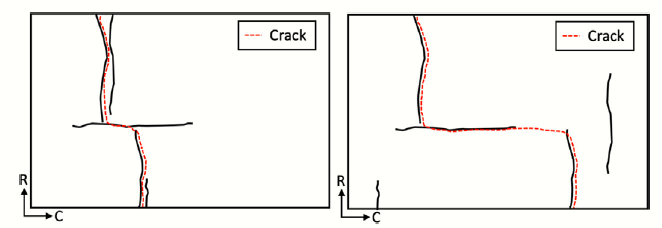
\includegraphics[width=4.3in]{Figures/1-Introduction/same RHF.png}
    \caption{Same hydrides located differently: The same RHF value but different alignment \cite{SIMON2021152817}.}
    \label{fig:RHF_comparison}
\end{figure}

\vspace{0.1 in}

\subsection{Parameters calculation}


\noindent
RHF corresponds to the weight average of hydride length multiplied by a weighting factor. The formula employed is described below:


\begin{equation} \label{RHF_eqn}
RHF =  \frac{\sum_i L_i f_i }
            {\sum_i L_i}
\end{equation}


\noindent
Where $L_i$ is the length of each hydride and $f_i$ is the weighting factor, a parameter that has different values depending on the hydrides orientation. Hydrides with orientations between 0-40° to the transverse direction have a $f_i$ of 0, when the orientation is between 40° and 65°, the $f_i$ is 0.5, and hydrides with an orientation of 65–90° have a $f_i$ of 1 \cite{COLAS2013586}. 

\noindent
To calculate the HCC, a rectangular area in the micrograph of the alloy is separated, and the length of each radial hydride in that area is measured. The formula applied is shown below:

\begin{equation} \label{HCC_eqn}
HCC =  \frac{HC_1 + HC_2 + HC_3... }
            {L}
\end{equation}

\noindent
Where $HC_i$ is the length of each radial hydride and L is the height of the selected rectangle to measure \cite{SIMON2021152817}.

\noindent
To calculate the RHCF, the length of each radial hydride in a section of the cladding is measured. This time, the section will have a length of 150 µm along the arc length of the cladding, and the width will be all the cladding thickness. The formula applied in this case is:

\begin{equation} \label{RHCF_eqn}
RHCF =  \frac{max (L_1 + L_2 + L_3...) }
            {h_m}
\end{equation}

\noindent
Where $L_i$ is the length of each radial hydride within the 150 µm of arc length, and $h_m$ is the cladding thickness \cite{SIMON2021152817}.

In Figure \ref{fig:parameters_drawing}, there is a drawing where the calculations of the HCC (a) parameter and the RHCF parameter (b) are illustrated.

\begin{figure}[h] %  figure placement: here, top, bottom, or page
    \centering
    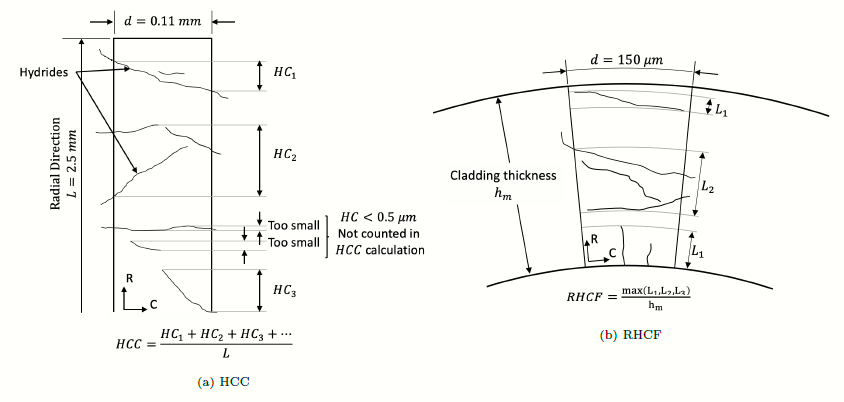
\includegraphics[width=5.5in]{Figures/2-Parameters/parameters_drawing.png}
    \caption{Drawing of hydride platelets, showing how to calculate the parameters a) HCC, b) RHCF \cite{SIMON2021152817}.}
    \label{fig:parameters_drawing}
\end{figure}
\vspace{0.1 in}
\subsection{Limitations of each parameter}

\noindent
The problem of the RHF is that it does not differentiate between hydrides oriented within the ranges 0-40°, 40-65°, and 65-90° \cite{SIMON2021152817}. Thus, microstructures with different radial hydrides orientations can have the same $f_i$, which will lead to obtain the same value of RHF.

\noindent
The continuity factors do not differentiate some situations either. For example, the HCC is the same in the three situations illustrated in Figure \ref{fig:limitationhcc}, which certainly facilitate the cracking propagation to different extents. In Figure \ref{fig:limitationrhcf} it can be seen that two different situations entail the same value of RHCF and, on the contrary, Figure \ref{fig:sameconnectivity} shows how two equivalent situations may lead to different values of RHCF \cite{SIMON2021152817}.

\begin{figure}[h] %  figure placement: here, top, bottom, or page
    \centering
    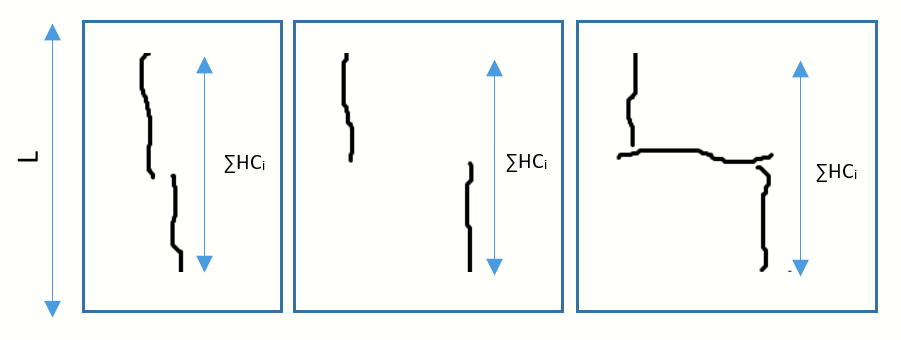
\includegraphics[width=4.5in]{Figures/3-Limitations/HCC comparison.png}
    \caption{Radial-oriented hydrides differently located but with the same HCC value.}
    \label{fig:limitationhcc}
\end{figure}

\begin{figure}[h] %  figure placement: here, top, bottom, or page
    \centering
    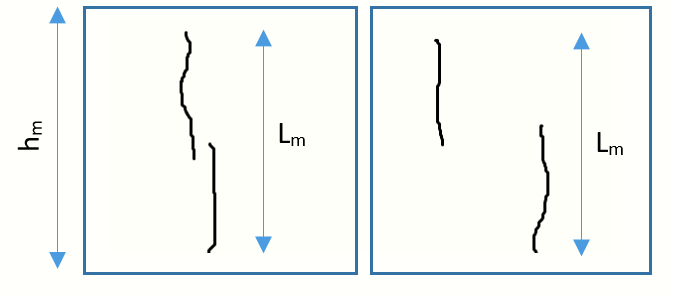
\includegraphics[width=4.5in]{Figures/3-Limitations/RHCF comparison 1.png}
    \caption{Radial-oriented hydrides with the same RHCF value but different connectivity.}
    \label{fig:limitationrhcf}
\end{figure}

\begin{figure}[h] %  figure placement: here, top, bottom, or page
    \centering
    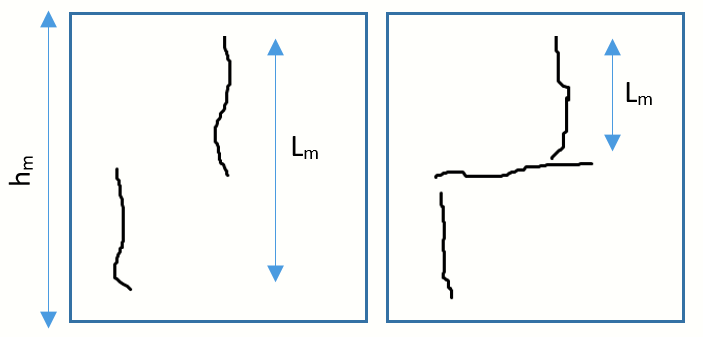
\includegraphics[width=4.5in]{Figures/3-Limitations/RHCF comparison 2.png}
    \caption{Radial-oriented hydrides with the different RHCF value but the same connectivity.}
    \label{fig:sameconnectivity}
\end{figure}

\vspace{0.1 in}
%========= Literature review
\section{Literature review}

\noindent
A.T. Motta et al. \cite{MOTTA} stated that, as hydrides orientation has a significant impact on the mechanical response of the cladding material, the modelling of hydride precipitation and dissolution should cover not only the volume fraction of the precipitated hydrides, but also their morphology. They said that the presence of radial hydride particles has a direct influence on crack propagation, since it provides an energetically favourable fracture path through the cladding wall, whereas circumferential hydrides interferes to a small extent. However, when different thermo-mechanical processes are applied, hydrides can evolve from a circumferential to radial orientation, which reduces the overall strength of the cladding. They pointed as an important research need to establish the limits at which the created hydride microstructure significantly affect cladding ductility.

\noindent
R.K. Sharma et al. \cite{SHARMA2018546} studied the propagation of cracks in  Zr-2.5\%Nb samples with hydrides in their microstructure. By applying annealing, they decreased the value of HCC, and this improves the fracture resistance of the material. In Figure  \ref{fig:ref2}, it can be seen how the fracture toughness $(KJ_{max})$ increases when HCC is smaller, and how it reaches extremely high values when HCC is near 0.

\begin{figure}[h] %  figure placement: here, top, bottom, or page
    \centering
    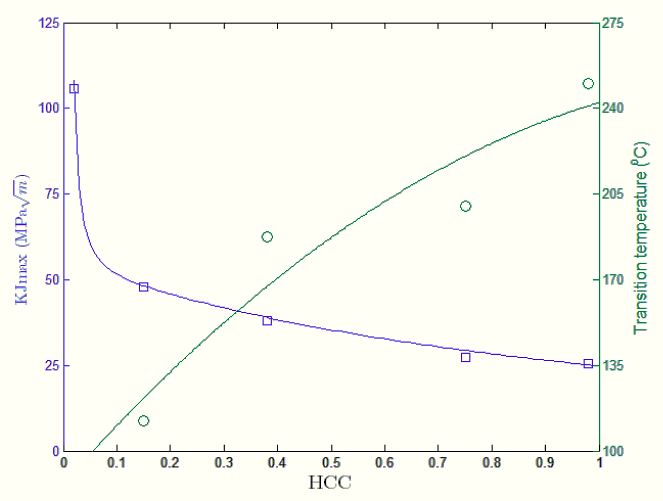
\includegraphics[width=3.8in]{Figures/4-Lit. Review/HCCref2.png}
    \caption{Fracture toughness $(KJ_{max})$ at room temperature and transition temperature evolution with respect to HCC \cite{SHARMA2018546}.}
    \label{fig:ref2}
\end{figure}

\noindent
S. Sunil et al. \cite{SUNIL} studied the Delayed Hydride Cracking (DHC) on the same alloy, Zr-2.5\%Nb. The material had a radial hydrides presence corresponding to a mean HCC value of around 0.8 at room temperature. After heating the samples at 200 and 225°C, their HCC value lowed to 0.576 and 0.44, respectively. They showed schematically (see Fig. \ref{fig:ref3}) how a crack propagates linearly when there are longitudinal hydrides (low HCC) and in zig-zag when there are radial hydrides (high HCC).

\begin{figure}[h] %  figure placement: here, top, bottom, or page
    \centering
    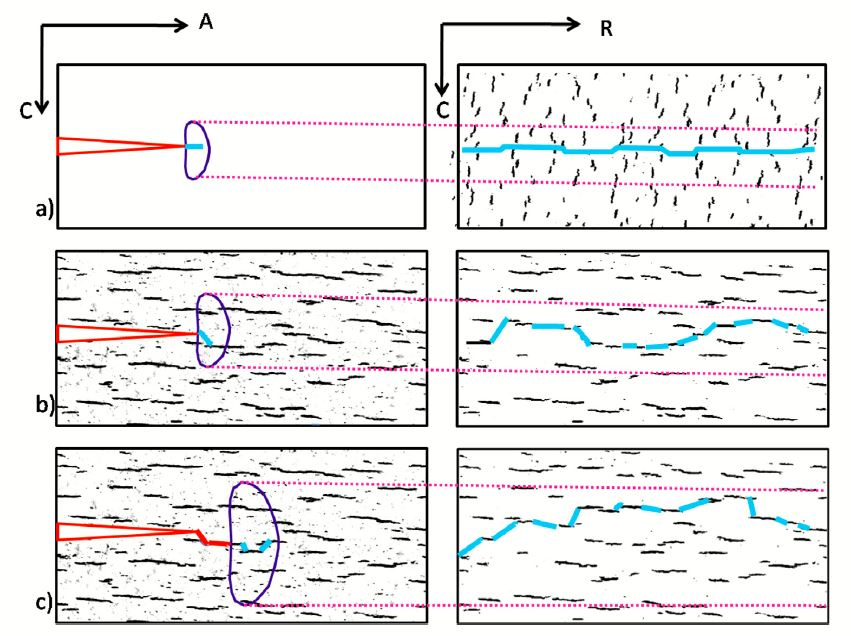
\includegraphics[width=4.4in]{Figures/4-Lit. Review/propagation.JPG}
    \caption{Crack propagation a) In presence of longitudinal hydrides (planar propagation), b and c) In presence of radial hydrides, before and after crack propagation (zig-zag propagation)  \cite{SUNIL}.}
    \label{fig:ref3}
\end{figure}


\noindent
In his PhD dissertation in Nuclear Engineering, P.C. Simon \cite{thesis} designed with MATLAB a tool to obtain automatically metrics to quantify hydride microstructure in 2D images and relate them with crack propagation. He verified  his method on schematic micrographs with known expected values. This tool can be downloaded from: https://github.com/simopier/QuantifyingHydrideMicrostructure. 


\vspace{0.1 in}
\noindent
By following a similar schema, in this project it was developed a model that reads a Zr-alloy microstructure and  returns its HCC value to evaluate the hydride connectivity.


\vspace{0.1 in}
%========= Methodology
\section{Methodology \& Discussion}

In this work, three types of thresholding was performed: Otsu, K-means and Gaussian. The HCC was calculated for all of them to check which method is the most accurate in terms of hydrides connectivity evaluation. Using GitHub to collaborate, we developed a Jupyter notebook from which the functions are called to show clarity in the script.

\noindent
The following sections were developed throughout the workflow:

\begin{enumerate}

    \item \textbf{Import packages.}
This sections is used to call all the packages needed to the correct running of the whole script.

    \item\textbf{ Import the images from GitHub.}
In this part of the code, the images to analyse are loaded.

    \item \textbf{Image processing.}
Because of the large area of the images being analysed, there are shadows that may lead us to incorrect results. To solve this, here it is included some code to break the image into vertical grayscale strips. The strips are also blurred and saved in their own directories.

    \item \textbf{Thresholding.}
In this part, the grayscale and blurred strips are transformed into binary images and three different thresholding methods are applied to see which one offers the best result:

\begin{itemize}
\item \textbf{Otsu thresholding}
\end{itemize}

\begin{itemize}
\item \textbf{K-means thresholding}
\end{itemize}

\begin{itemize}
\item \textbf{Thresholding - Gaussian}
\end{itemize}

Adaptive Gaussian thresholding was applied to binarize the image. Adaptive means that the levels for each thresholded pixel were chosen based on the surrounding pixels, in order to adapt the thresholding according to different levels of illumination or contrast on the image. Unfortunately, due to the complexity of the images and very different illumination conditions across the whole sample size, the result from adaptive Gaussian thresholding was extremely noisy and therefore, unsuitable for HCC analysis.

To mitigate this, erosion and dilation treatments were employed (provided by OpenCV), as well as area-based thresholding (removed an isolated island of pixels below a specified area threshold) (provided by skimage). Both methods were also combined for the sake of comparison. An example of what was obtained is shown in Figure X.

Based on qualitative analysis, the erosion and dilation treatment did very little on its own to improve the presence of noise on the binarized micrographs. The area-based thresholding had far greater success, with the connected hydride structures present in the original images becoming more clearly visible. Combining both treatments offered an improvement for images with more initial noise, but removed long hydrides for images with less initial noise. At this time, a method has not been developed that uses the best method for the appropriate image. Therefore, for any set of images, the method would have to be chosen qualitatively for each image. Hence, this method is too inconsistent to be considered useful for HCC analysis. 

    \item \textbf{Connectivity of microstructure.}
In this section, the connectivity between hydrides in the radial direction and the edges are detected to discover the contours within the slices. With this information, the HCC parameter of each strip is measured, and finally the average HCC value is obtained for each of the three thresholding methods.

    \item \textbf{Testing of functions.}
Testing the code in each function allows for a more robust execution of the code by integrating and automating the test procedure. Example micrographs created and modified with known will enable us to know what outputs to expect for each function's input. Comparing the similarity of images gives us a pass or fail criteria.By anticipating how the end-user might use the code and its environment, testing decreases the likelihood of unexpected errors. \par

Description of test methods:

\begin{itemize}


\item Processing: 
 
            \begin{figure}[h] 
            \centering
            
\includegraphics[width=2in]{Figures/testing/45Degrees.png}
            \caption{Test image with of 889 png by 500 png}
            \label{fig:processing_vertical_strips}
            \end{figure}   


    A test was made to check vertical strips produced in the program. The vertical strips function is one of the most important functions which enables the rest of the functions to work.
    Figure \ref{fig:processing_vertical_strips} was used with dimensions of 889 x 500 png. Processing.vertical\_strips() sections the image into equal sections by dividing the image width by an integer starting from 15. The function should only return the number 7. If it doesn't there is a problem with the code. 
    \item Connectivity:
    
    Connectivity.otsu() transforms grey-scale image like Figure \ref{fig:gradient_in} to a black and white image, Figure \ref{fig:Grad_Out}. By comparing the Numpy data array of the we can check the efficacy of the function.
    
    
    \noindent
        \begin{figure}
             \centering
             \begin{subfigure}[b]{0.3\textwidth}
                 \centering
                 
\includegraphics[width=\textwidth]{Figures/testing/Gradient.png}
                 \caption{Light to dark gradient used for testing thresholding calculation}
                 \label{fig:gradient_in}
             \end{subfigure}
             
             \begin{subfigure}[b]{0.3\textwidth}
                 \centering
                 
\includegraphics[width=\textwidth]{Figures/testing/Gradient_out.png}
                 \caption{Output image for test gradient}
                 \label{fig:Grad_Out}
             \end{subfigure}
            
            \caption{Input and Output Images for thresholding test}
            \label{fig:two gradients}
        \end{figure}
    
    \item Parameters:
        One of the main aims of the code was to find the Hydride Continuity factor of micrographs produced. Figure \ref{fig:test_image_hcc2} was the image chosen to check HCC value. By substituting the length of each hydride and total length of the strip in equation \ref{HCC_eqn} , equation \ref{test_hcc_eqn} is produced. This gives the expected return value of the HCC function when Figure \ref{fig:test_image_hcc2} is used.
        
        \begin{figure}[h] 
        \centering
        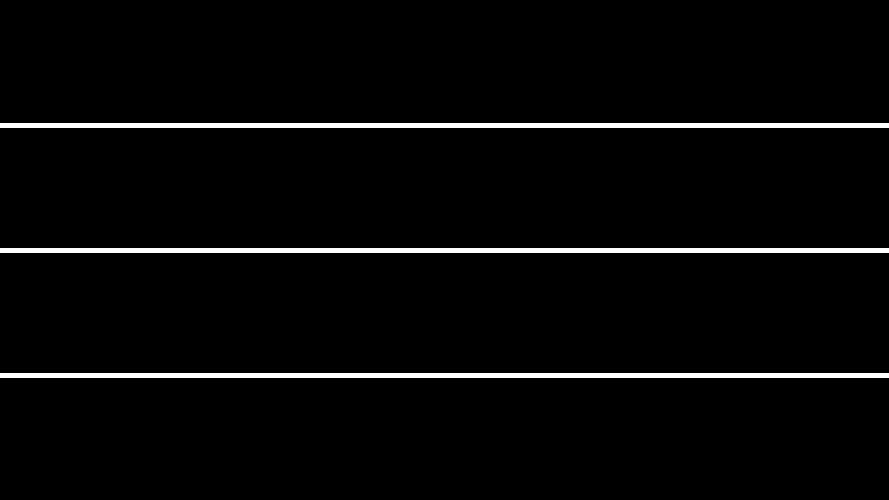
\includegraphics[width=2in]{Figures/testing/Full_Horizontal.png}
        \caption{Image to test HCC2 function}
        \label{fig:test_image_hcc2}
        \end{figure}
        
        \begin{equation} \label{test_hcc_eqn}
        \frac{3.68 + 3.68 + 3.68 }
                {133.86}
        = 0.0824742268
        \end{equation}
    
    \item For Gaussian thresholding two tests were created:
    
    \begin{enumerate}
        \item Tests whether after each treatment the input image and the output image had at least a 95\% similarity in terms of the image arrays. The test(s) was made to quickly determine whether a treatment (or its chosen parameters) had a large enough effect on the image to be considered useful.
        \item After the initial adaptive Gaussian thresholding, each pixel of the image was analyzed to determine whether it was white (value of 0) or black (value of 255). The test was made to confirm that the binarization had been successful and whether any possible subsequent treatment can rely on the fact the image is truly binary.
    
    \end{enumerate}
\end{itemize}


\end{enumerate}



\vspace{0.1 in}
\section{Results \& Discussion}

\begin{figure}[h] %  figure placement: here, top, bottom, or page
    \centering
    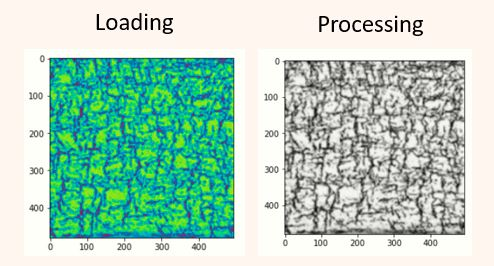
\includegraphics[width=4.5in]{Figures/4-Results/loading&processing.JPG}
    \caption{Image to be analysed, before and after processing.}
    \label{fig:limitationrhcf}
\end{figure}


\begin{figure}[h] %  figure placement: here, top, bottom, or page
    \centering
    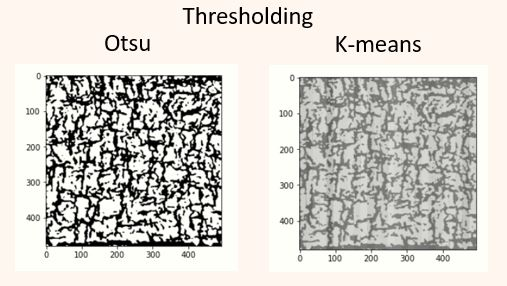
\includegraphics[width=4.5in]{Figures/4-Results/thresholding.JPG}
    \caption{Images after two different thresholds are applied: a) Otsu b) K-means.}
    \label{fig:limitationrhcf}
\end{figure}


\begin{figure}[h] %  figure placement: here, top, bottom, or page
    \centering
    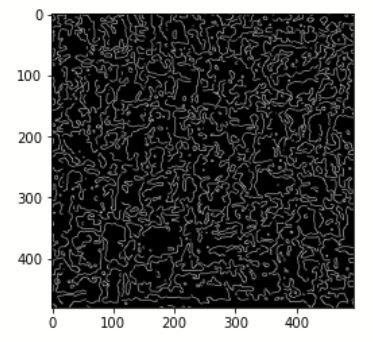
\includegraphics[width=2.5in]{Figures/4-Results/Otsu.JPG}
    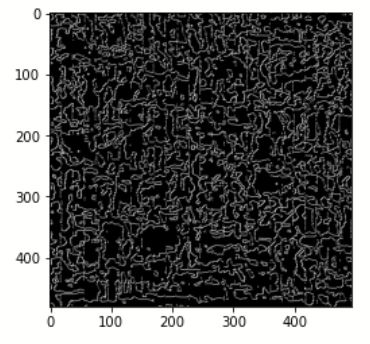
\includegraphics[width=2.5in]{Figures/4-Results/k-means.JPG}
    \caption{Connectivity of the images with a) Otsu threshold, b) K-means threshold.}
    \label{fig:limitationrhcf}
\end{figure}


\vspace{0.1 in}
%========= Conclusions

\section{Conclusions \& Future Work}


\newpage
\singlespacing
\bibliography{biblography}
\bibliographystyle{IEEEtran}

\end{document}